\subsection{Используемые алгоритмы}

\subsubsection{Кластеризация}

Для идентификации принадлежности элемента к кластеру используется алгоритм Хошена-Копельмана \cite{hoshen}, который был модифицирован под континуальную задачу. 

За один проход данный алгоритм идентифицирует все кластеры и определяет распределение элементов по кластерам. Используются следующие обозначения: $k$ — номер кластера, $nec[i]$ — кластерная метка $i$-ого элемента, $kk[k]$ — размер $k$-то кластера. Используется понятие соседи: для случая окружностей в задаче узлов соседями являются такие сферы, центры которых находятся на расстоянии, равном или меньшим $2(r + coef)$; для случая сфер в смешанной задаче соседями являются такие сферы, центры которых находятся на расстоянии, равном или меньшим $2 (г + coef)$; для случая эллипсоидов соседями являются такие эллипсоиды, оболочки которых пересекаются. Для проверки пересечения проницаемых оболочек в классе каждого элемента, с которым работает библиотека, должна присутствовать функция $object.is\_intersect(other\_object)$, которая должна возвращать положительный результат в случае, если элементы $object$ и $other\_object$ пересекаются. 

Подход с использованием функцкии, определяющей пересечение элементов в классе исследуемого обьекта, позволяет библиотеке использовать любые типы объектов. Для добавления в программу расчёта порога перколяции для квадратов, достаточно создать класс $Square()$, определить его основные параметры, добавить функцию $is\_intersect(other\_object)$, а также добавить функцию $try\_to\_move$, которая будет использоваться при попытках переместить элемент в процессе перемешивания.

Алгоритм работает по следующей схеме: 
\begin{enumerate}
    \item При генерации первого элемента ему присваивается кластерная метка $1$ и размеру первого кластера также присваивается значение $1$. 
    \item Для каждого следующего элемента $i$, где $2 \leq г \leq п$, проверяется, существуют ли среди ранее проверенных элементов (уже имеющих кластерную метку) ее соседи.
    \item Если соседей не нашлось, то элемент $i$ предположительно принадлежит новому кластеру. В этом случае $k$ увеличивается на $1$, элементу $i$ присваивается $k$-ое значение кластерной метки и значению размера $k$-ro кластера присваивается $1$. 
    \item Если встречается один сосед, то два элемента принадлежат одному кластеру. В этом случае элементу $i$ присваивается кластерная метка соседа и размер кластера с данной меткой увеличивается на $1$. 
    \item Если соседей нашлось несколько, то все элементы принадлежат одному кластеру. В этом случае, соседи могут иметь как одинаковые, так и разные кластерные метки. Если все кластерные метки соседей одинаковые, то сфере $i$ присваивается кластерная метка соседа и размер кластера с данной меткой увеличивается на $1$. Если среди соседей есть такие, которые имеют разные кластерные метки, то возникает конфликт кластерных меток. В этом случае: 
    \begin{enumerate}
        \item находим среди кластерных меток наименьшую, она является правильной кластерной меткой, остальные метки являются неправильными; 
        \item элементу $i$ и всем соседям присваивается значение правильной кластерной метки, размер кластера с правильной меткой увеличивается на $(1+(количество соседей—1))$; 
        \item среди ранее рассмотренных элементов находятся те, которые имеют неправильные кластерные метки. Для каждого такого элемента меняем кластерную метку на правильную, размер кластера с правильной меткой увеличивается на количество таких элементов, а размеры кластеров с неправильными кластерными метками обнуляются. 
    \end{enumerate}
\end{enumerate}

Модифицированный алгоритм Хошена-Копельмана отличается от классического тем, что в классическом алгоритме перебираются по порядку все слои решетки, а в модифицированном перебираются все элементы от 1 до п. Это даст возможность работать алгоритму не на решетке, а в континууме. Кроме того, при работе данного алгоритма создаются списки соседей для каждого элемента. Таким образом, при выполнении модифицированного алгоритма Хошена-Копельмана каждому элементу присваивается кластерная метка. Известно распределение элементов по кластерам, то есть мы знаем сколько существует кластеров и размер каждого кластера. 


\subsection{Перколяционные свойства случайного ансамбля при различных параметрах частиц}

Для описания значительно большего спектра различных физических процессов, следует перейти от исследования задач на решётке к контируальным задачам, в которых, в отличие от первых координаты элементов принимают не дискретные, а непрерывные значения. Такой подход позволяет добиться максимального приближения к зачастую бесформенным структурам, которые наблюдаются в реальных физических процессах.

Для описания ряда физических явлений, наилучшим приближением является приближение, в котором элементы представляют собой вытянутые эллипсы, поэтому в библиотеке присутствует отдельный раздел, посвящённый генерации и исследованию перколяционных свойств на эллипсоидах.



\newcommand{\imgsize}{9cm}
\renewcommand{\imgsubdir}{percolation/ellipce}
\begin{figure}[h!]
    \begin{subfigure}{0.49\textwidth}
        \centering
        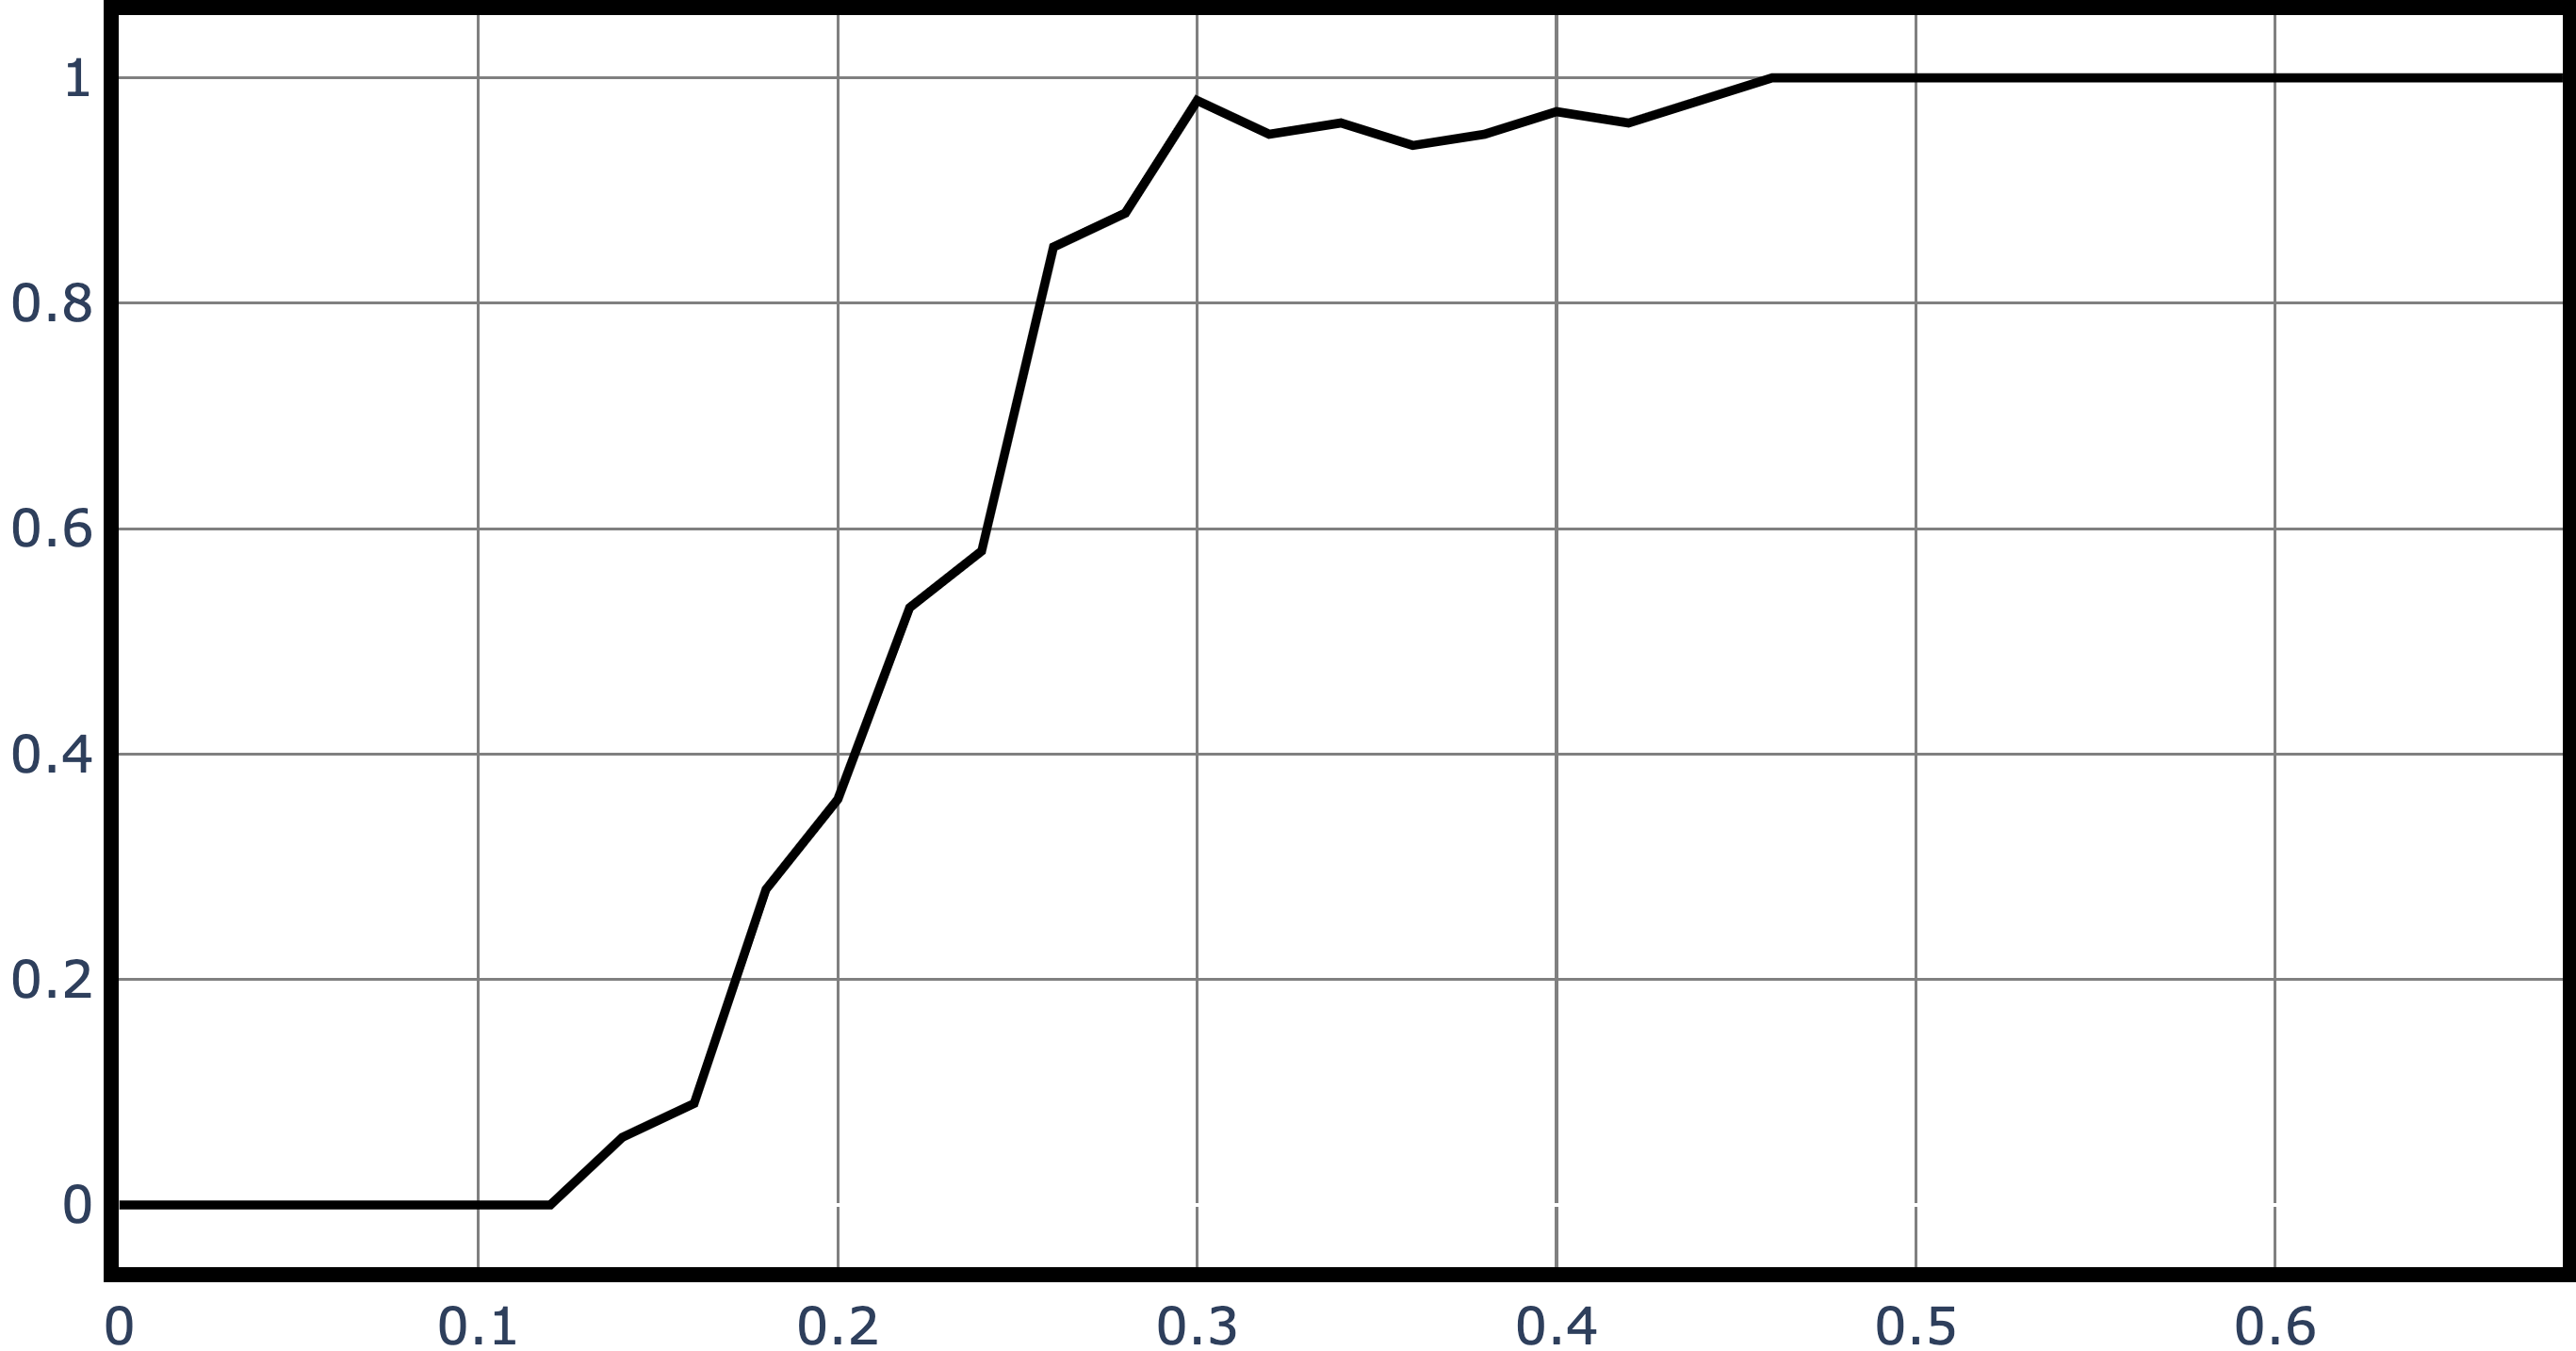
\includegraphics [width=\textwidth,height=\imgsize]
        {figures/\imgsubdir/e086.png}
        \caption{Параметр эксцентриситета $0.86$}
    \end{subfigure}
    \begin{subfigure}{0.49\textwidth}
        \centering
        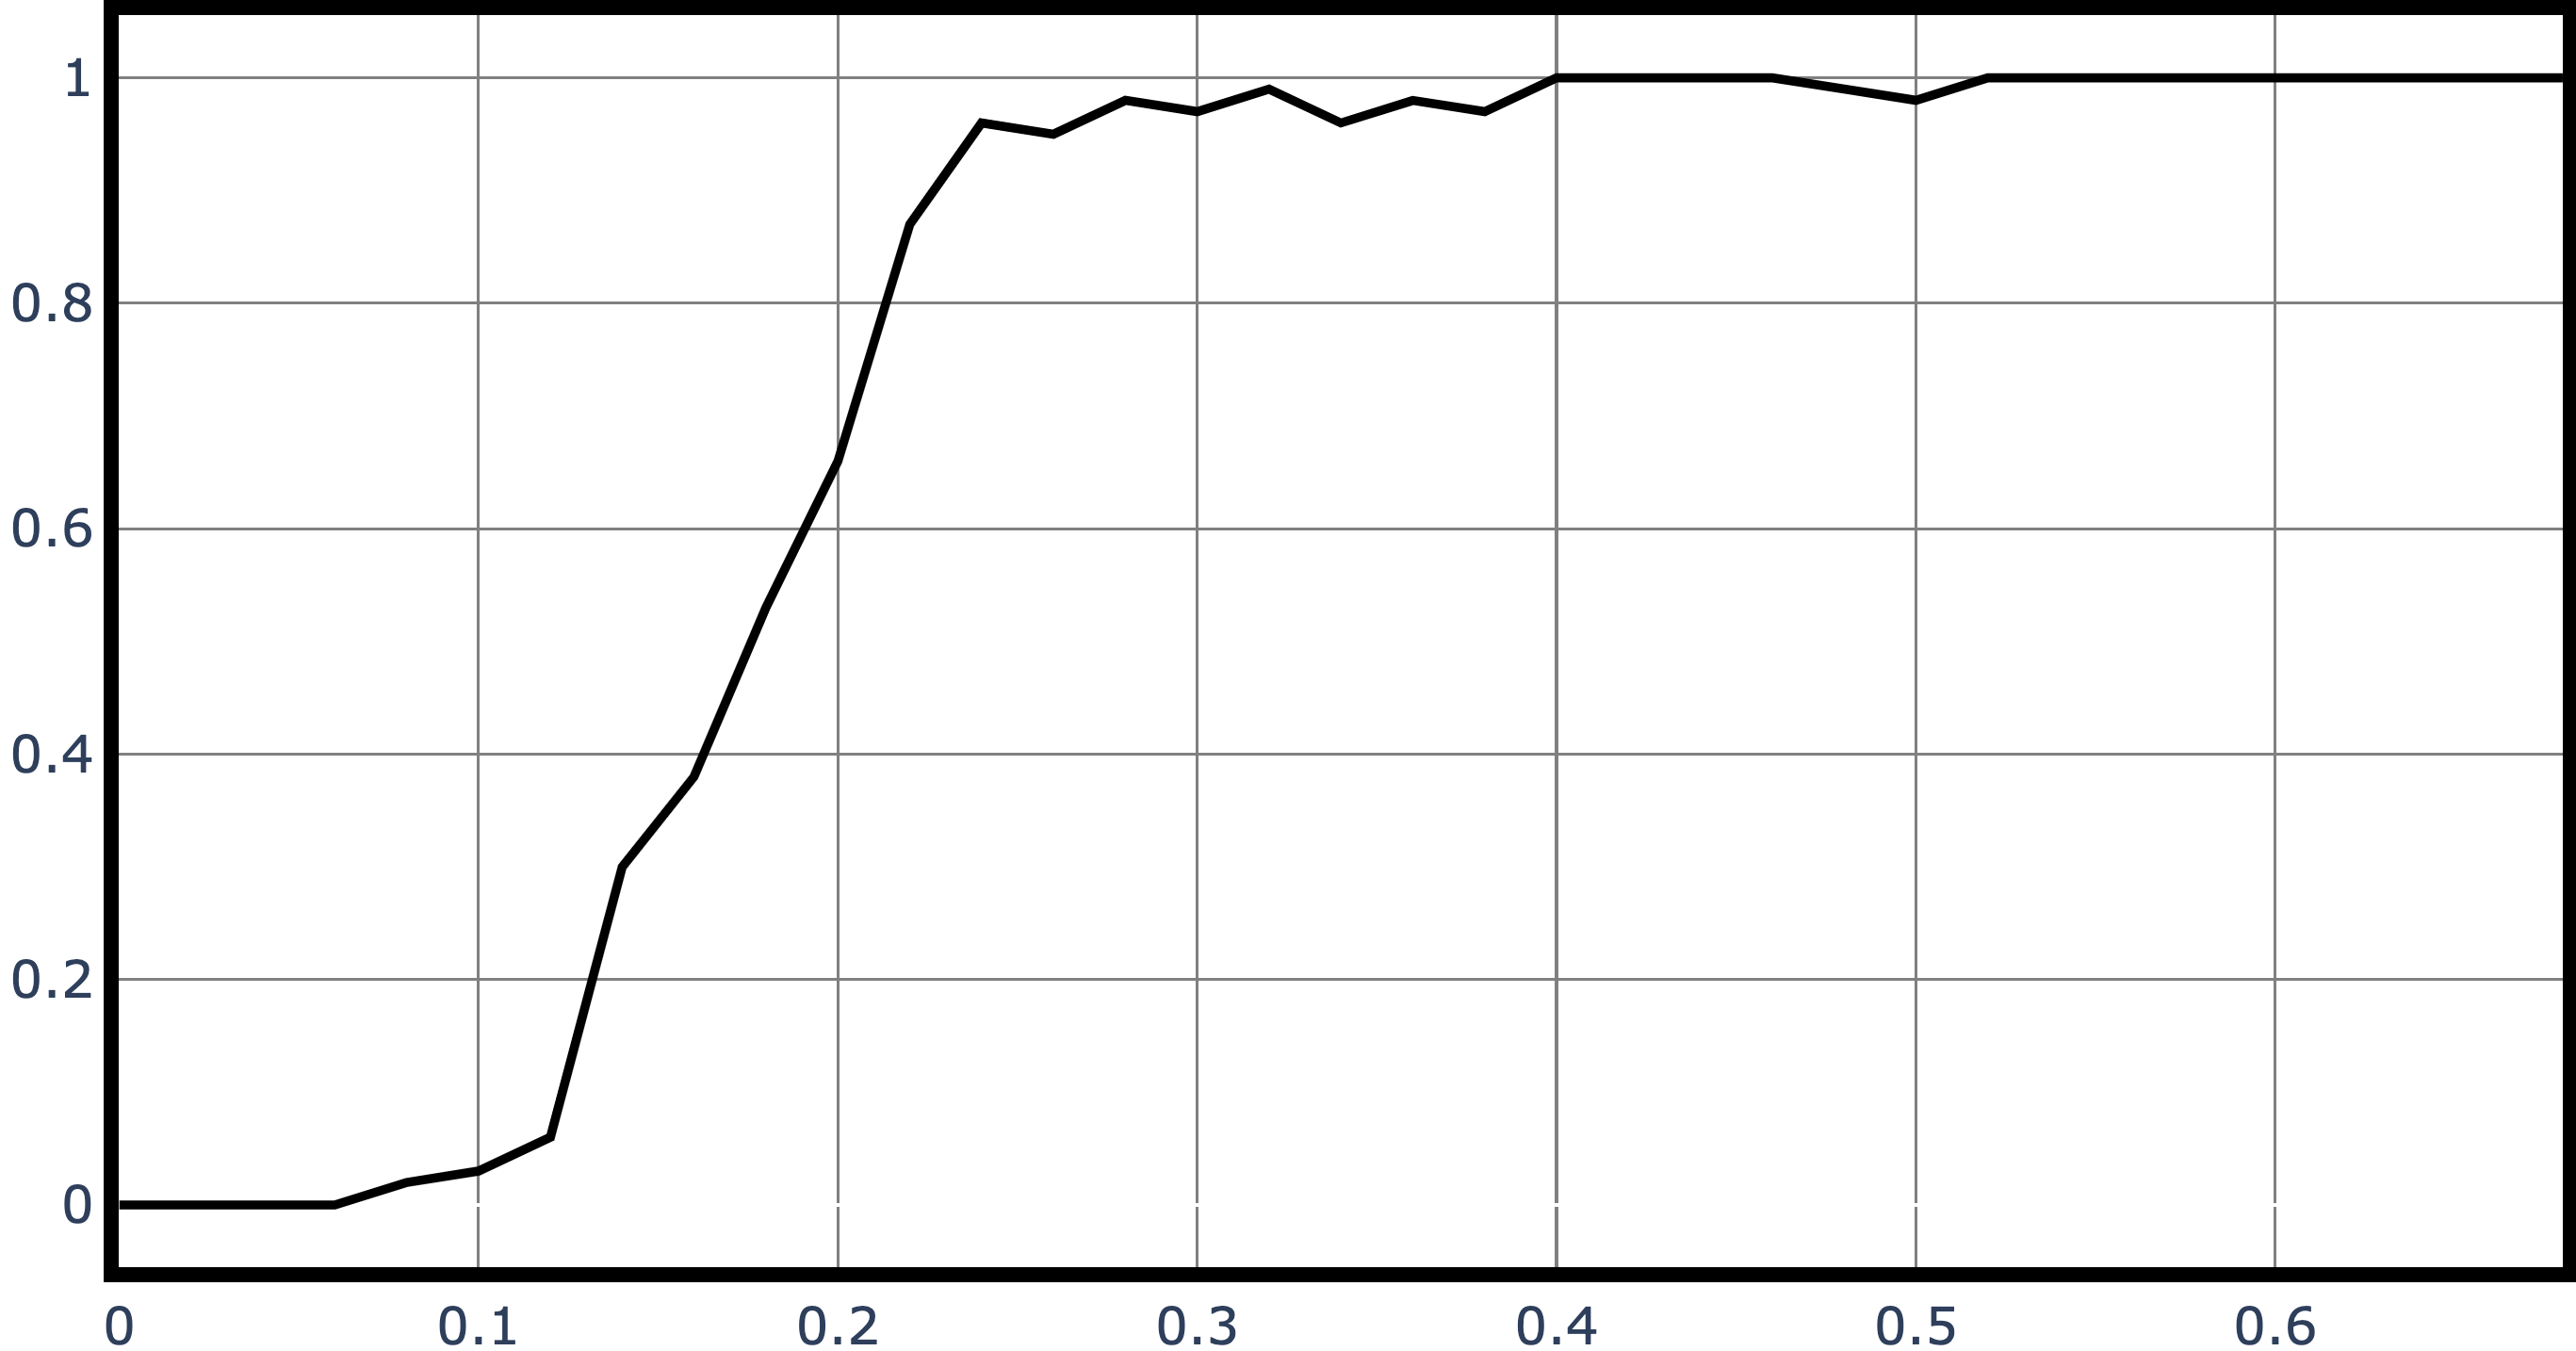
\includegraphics [width=\textwidth,height=\imgsize]
        {figures/\imgsubdir/e097.png}
        \caption{Плотность заполнения $0.97$}
    \end{subfigure}
    \caption{Зависимость вероятности появления проводящего кластера от процента заполненности пространства.}
    \label{fig:tight_packing}
\end{figure}

Как показано на данных рисунках, библиотека позволяет с высокой точностью определить местоположение порога перколяции.

\subsection{Расчёт перколяционных характеристик на случайных ансамблях при различной форме частиц}

